\documentclass{exercise_wvqusrai}
% 设置表头、表尾
\lhead{\yy 学号\,\fillin}
\chead{\yy 姓名\,\fillin}
\cfoot{}
\rhead{\li 衡阳师范学院数学组}
\geometry{voffset=0.5in}
\begin{document}
\begin{questions}
\dati{一}{选择题}
\question[4]
$\overrightarrow{CB}+\overrightarrow{AD}+\overrightarrow{BA}=(\qquad)$

\begin{oneparchoices}
\choice $\overrightarrow{DB}$
\choice $\overrightarrow{BA}$
\choice $\overrightarrow{CD}$
\choice $\overrightarrow{DC}$
\end{oneparchoices}

\question[4]
已知$\vec{a}=\begin{pmatrix}
-1\\2
\end{pmatrix},\vec{b}=\begin{pmatrix}
3\\1
\end{pmatrix}$.则$\left(\vec{a}+\vec{b}\right)\cdot\left(\vec{b}-\vec{2a}\right)=(\qquad)$

\begin{oneparchoices}
\choice 1
\choice 19
\choice 7
\choice -1 
\end{oneparchoices}


\question[4]
设$\vec{a}=\begin{pmatrix}
\frac{3}{2}\\
\sin\alpha
\end{pmatrix},\vec{b}=\begin{pmatrix}
\cos\alpha\\
\frac{1}{3}
\end{pmatrix}$,且$\vec{a}\sslash\vec{b}$,则锐角$\alpha=(\qquad)$

\begin{oneparchoices}
\choice $30^\circ$
\choice $45^\circ$
\choice $60^\circ$
\choice $75^\circ$
\end{oneparchoices}

\question[4]
若$\left|\overrightarrow{AB}\right|=\left|\overrightarrow{AD}\right|$,且$\overrightarrow{BA}=\overrightarrow{CD}$,则四边形$ABCD$的形状为$(\qquad)$

\begin{oneparchoices}
\choice 平行四边形
\choice 矩形
\choice 菱形
\choice 等腰梯形
\end{oneparchoices}

\question[4]
已知非零向量$\vec{a},\vec{b}$满足$\left|\vec{a}\right|=2\left|\vec{b}\right|$,且$\left(\vec{a}-\vec{b}\right)\perp\vec{b}$,则$<\vec{a},\vec{b}>=(\qquad)$

\begin{oneparchoices}
\choice $\frac{\pi}{6}$
\choice $\frac{\pi}{3}$
\choice $\frac{2\pi}{3}$
\choice $\frac{5\pi}{6}$
\end{oneparchoices}

\fullwidth{\large \textbf{二、填空题}}
\question[5]
已知向量$\vec{a}=(-4,3),\vec{b}=(6,m)$,且$\vec{a}\perp\vec{b}$,则$m=\fillin$

\question[5]
已知$\vec{a}=\begin{pmatrix}
2\\3
\end{pmatrix},\vec{b}=\begin{pmatrix}
5\\6
\end{pmatrix}$,则$\left|\vec{a}-\vec{b}\right|=\fillin$

\question[5]
已知向量$\vec{a},\vec{b},\vec{c}$满足$\left|\vec{a}\right|=1,\left|\vec{b}\right|=2,\vec{c}=\vec{a}+\vec{b},\vec{c}\perp\vec{a}$,则$<\vec{a},\vec{b}> = \fillin$.

\question[5]
若$\overrightarrow{AB}=\frac{3}{5}\overrightarrow{BC}$,则$\overrightarrow{OB}=\fillin[][0.5in]\overrightarrow{OA}+\fillin[][0.5in]\overrightarrow{OC}$.

\fullwidth{\large \textbf{三、解答题}}
\question[15]
已知向量$\vec{a}=\begin{pmatrix}
1\\2
\end{pmatrix},\vec{b}=\begin{pmatrix}
2\\-2
\end{pmatrix}$,
\begin{parts}
\part 设$\vec{c}=4\vec{a}+\vec{b}$,求$\left(b-c\right)\cdot\vec{a}$;
\part 若$\vec{a}+\lambda\vec{b}$与$\vec{a}$垂直,求$\lambda$的值.
\end{parts}

\question[15]
平面直角坐标系$xOy$中,已知点$A(-1,2),B(2,3),C(-2,-1)$,
\begin{parts}
\part 分别计算$\overrightarrow{AB},\overrightarrow{AC},\overrightarrow{BC}$;
\part 求以线段$AB,AC$为邻边的平行四边形的两条对角线的长.
\end{parts}

\question[10]
已知$O=(0,0),A=(1,2),B=(3,4)$,请尽量尝试使用向量
\begin{parts}
\part 求$\cos\angle AOB$;
\part 计算$\Delta ABC$的面积.
\end{parts}

\question[20]
使用向量证明三角形的三条中线交于一点。
\begin{figure}[h]
    \centering
    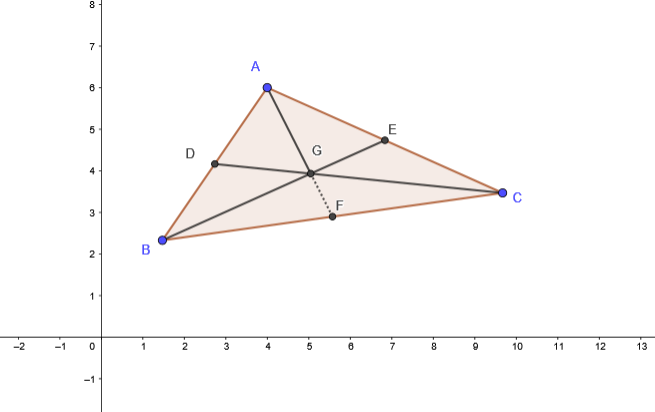
\includegraphics[width=5.2cm,keepaspectratio]{barycenter.PNG}
    \label{fig:geometric_barycenter}
\end{figure}
\end{questions}
\end{document}